\documentclass[1p]{elsarticle_modified}
%\bibliographystyle{elsarticle-num}

%\usepackage[colorlinks]{hyperref}
%\usepackage{abbrmath_seonhwa} %\Abb, \Ascr, \Acal ,\Abf, \Afrak
\usepackage{amsfonts}
\usepackage{amssymb}
\usepackage{amsmath}
\usepackage{amsthm}
\usepackage{scalefnt}
\usepackage{amsbsy}
\usepackage{kotex}
\usepackage{caption}
\usepackage{subfig}
\usepackage{color}
\usepackage{graphicx}
\usepackage{xcolor} %% white, black, red, green, blue, cyan, magenta, yellow
\usepackage{float}
\usepackage{setspace}
\usepackage{hyperref}

\usepackage{tikz}
\usetikzlibrary{arrows}

\usepackage{multirow}
\usepackage{array} % fixed length table
\usepackage{hhline}

%%%%%%%%%%%%%%%%%%%%%
\makeatletter
\renewcommand*\env@matrix[1][\arraystretch]{%
	\edef\arraystretch{#1}%
	\hskip -\arraycolsep
	\let\@ifnextchar\new@ifnextchar
	\array{*\c@MaxMatrixCols c}}
\makeatother %https://tex.stackexchange.com/questions/14071/how-can-i-increase-the-line-spacing-in-a-matrix
%%%%%%%%%%%%%%%

\usepackage[normalem]{ulem}

\newcommand{\msout}[1]{\ifmmode\text{\sout{\ensuremath{#1}}}\else\sout{#1}\fi}
%SOURCE: \msout is \stkout macro in https://tex.stackexchange.com/questions/20609/strikeout-in-math-mode

\newcommand{\cancel}[1]{
	\ifmmode
	{\color{red}\msout{#1}}
	\else
	{\color{red}\sout{#1}}
	\fi
}

\newcommand{\add}[1]{
	{\color{blue}\uwave{#1}}
}

\newcommand{\replace}[2]{
	\ifmmode
	{\color{red}\msout{#1}}{\color{blue}\uwave{#2}}
	\else
	{\color{red}\sout{#1}}{\color{blue}\uwave{#2}}
	\fi
}

\newcommand{\Sol}{\mathcal{S}} %segment
\newcommand{\D}{D} %diagram
\newcommand{\A}{\mathcal{A}} %arc


%%%%%%%%%%%%%%%%%%%%%%%%%%%%%5 test

\def\sl{\operatorname{\textup{SL}}(2,\Cbb)}
\def\psl{\operatorname{\textup{PSL}}(2,\Cbb)}
\def\quan{\mkern 1mu \triangleright \mkern 1mu}

\theoremstyle{definition}
\newtheorem{thm}{Theorem}[section]
\newtheorem{prop}[thm]{Proposition}
\newtheorem{lem}[thm]{Lemma}
\newtheorem{ques}[thm]{Question}
\newtheorem{cor}[thm]{Corollary}
\newtheorem{defn}[thm]{Definition}
\newtheorem{exam}[thm]{Example}
\newtheorem{rmk}[thm]{Remark}
\newtheorem{alg}[thm]{Algorithm}

\newcommand{\I}{\sqrt{-1}}
\begin{document}

%\begin{frontmatter}
%
%\title{Boundary parabolic representations of knots up to 8 crossings}
%
%%% Group authors per affiliation:
%\author{Yunhi Cho} 
%\address{Department of Mathematics, University of Seoul, Seoul, Korea}
%\ead{yhcho@uos.ac.kr}
%
%
%\author{Seonhwa Kim} %\fnref{s_kim}}
%\address{Center for Geometry and Physics, Institute for Basic Science, Pohang, 37673, Korea}
%\ead{ryeona17@ibs.re.kr}
%
%\author{Hyuk Kim}
%\address{Department of Mathematical Sciences, Seoul National University, Seoul 08826, Korea}
%\ead{hyukkim@snu.ac.kr}
%
%\author{Seokbeom Yoon}
%\address{Department of Mathematical Sciences, Seoul National University, Seoul, 08826,  Korea}
%\ead{sbyoon15@snu.ac.kr}
%
%\begin{abstract}
%We find all boundary parabolic representation of knots up to 8 crossings.
%
%\end{abstract}
%\begin{keyword}
%    \MSC[2010] 57M25 
%\end{keyword}
%
%\end{frontmatter}

%\linenumbers
%\tableofcontents
%
\newcommand\colored[1]{\textcolor{white}{\rule[-0.35ex]{0.8em}{1.4ex}}\kern-0.8em\color{red} #1}%
%\newcommand\colored[1]{\textcolor{white}{ #1}\kern-2.17ex	\textcolor{white}{ #1}\kern-1.81ex	\textcolor{white}{ #1}\kern-2.15ex\color{red}#1	}

{\Large $\underline{12a_{0444}~(K12a_{0444})}$}

\setlength{\tabcolsep}{10pt}
\renewcommand{\arraystretch}{1.6}
\vspace{1cm}\begin{tabular}{m{100pt}>{\centering\arraybackslash}m{274pt}}
\multirow{5}{120pt}{
	\centering
	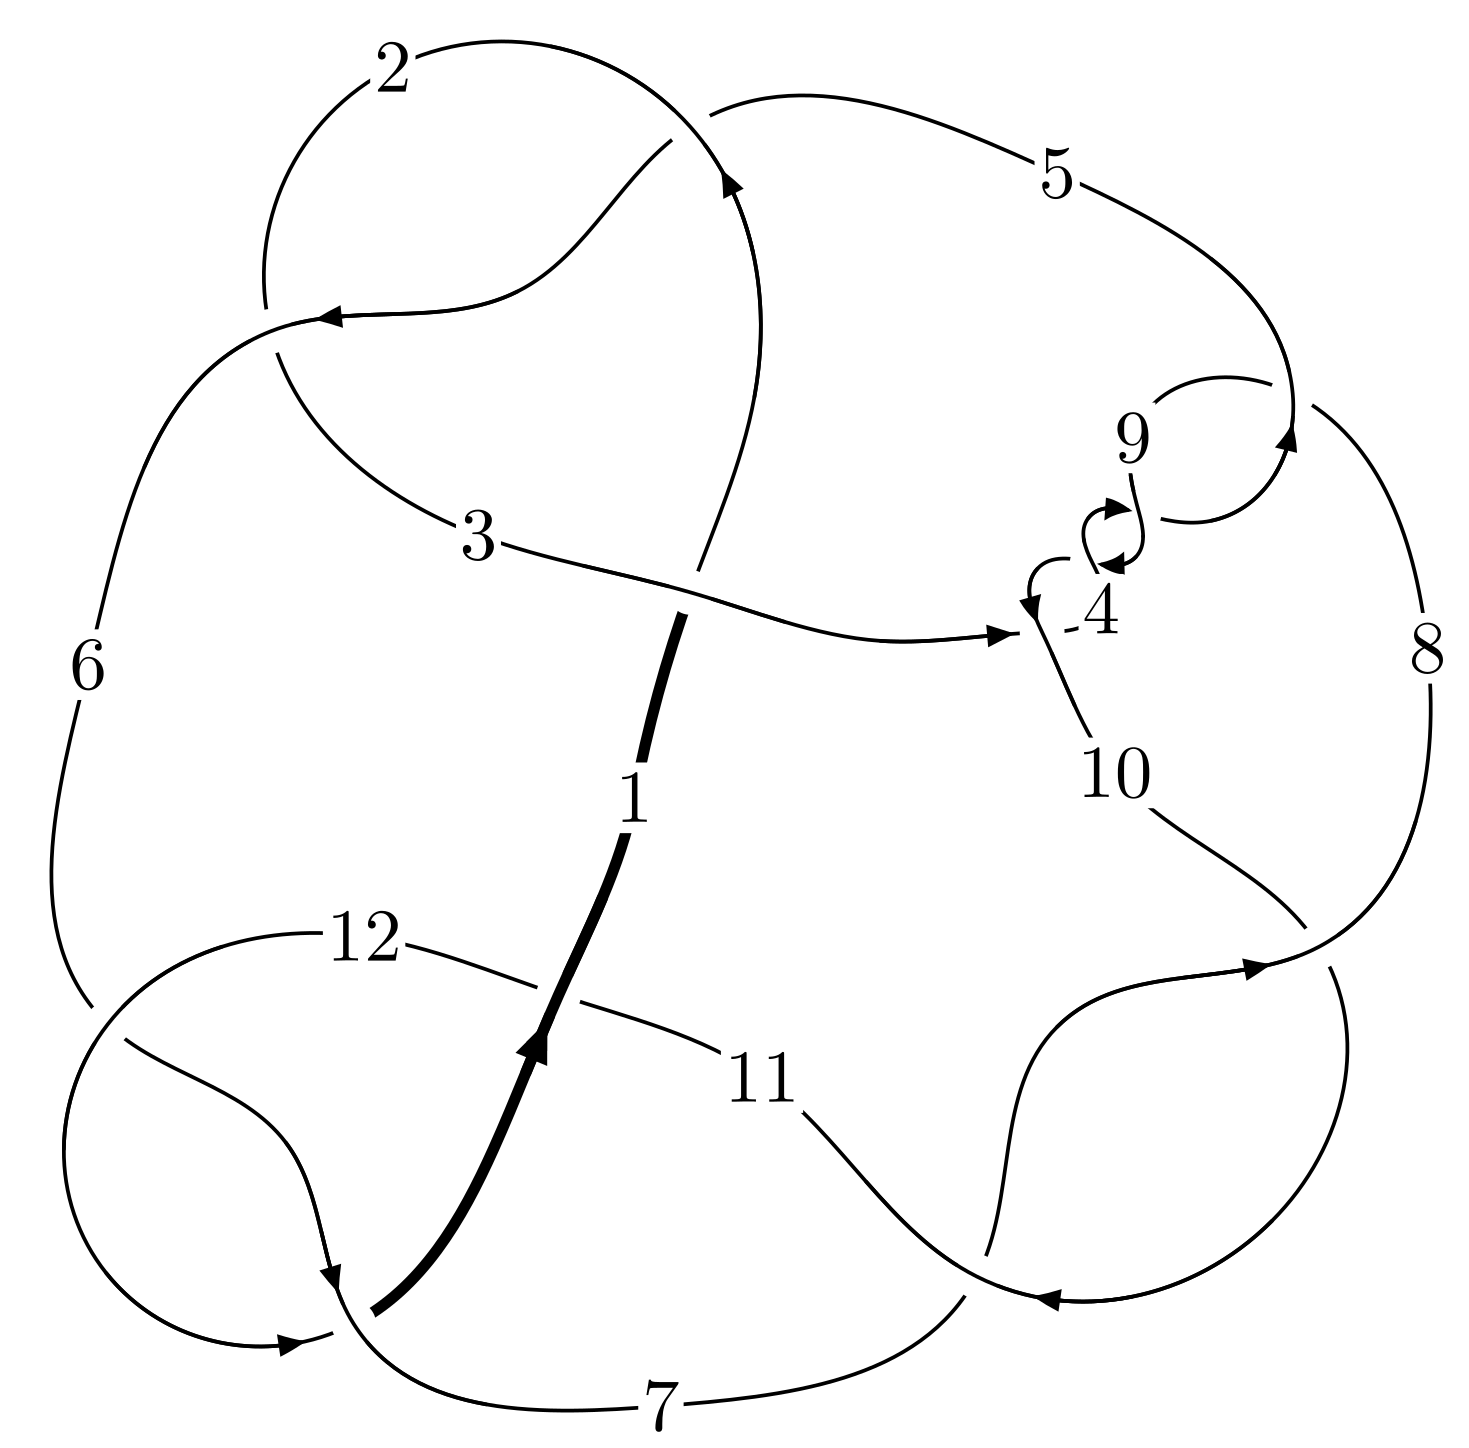
\includegraphics[width=112pt]{../../../GIT/diagram.site/Diagrams/png/1245_12a_0444.png}\\
\ \ \ A knot diagram\footnotemark}&
\allowdisplaybreaks
\textbf{Linearized knot diagam} \\
\cline{2-2}
 &
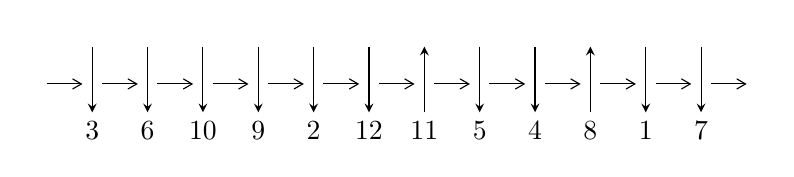
\begin{tikzpicture}[x=20pt, y=17pt]
	% nodes
	\node (C0) at (0, 0) {};
	\node (C1) at (1, 0) {};
	\node (C1U) at (1, +1) {};
	\node (C1D) at (1, -1) {3};

	\node (C2) at (2, 0) {};
	\node (C2U) at (2, +1) {};
	\node (C2D) at (2, -1) {6};

	\node (C3) at (3, 0) {};
	\node (C3U) at (3, +1) {};
	\node (C3D) at (3, -1) {10};

	\node (C4) at (4, 0) {};
	\node (C4U) at (4, +1) {};
	\node (C4D) at (4, -1) {9};

	\node (C5) at (5, 0) {};
	\node (C5U) at (5, +1) {};
	\node (C5D) at (5, -1) {2};

	\node (C6) at (6, 0) {};
	\node (C6U) at (6, +1) {};
	\node (C6D) at (6, -1) {12};

	\node (C7) at (7, 0) {};
	\node (C7U) at (7, +1) {};
	\node (C7D) at (7, -1) {11};

	\node (C8) at (8, 0) {};
	\node (C8U) at (8, +1) {};
	\node (C8D) at (8, -1) {5};

	\node (C9) at (9, 0) {};
	\node (C9U) at (9, +1) {};
	\node (C9D) at (9, -1) {4};

	\node (C10) at (10, 0) {};
	\node (C10U) at (10, +1) {};
	\node (C10D) at (10, -1) {8};

	\node (C11) at (11, 0) {};
	\node (C11U) at (11, +1) {};
	\node (C11D) at (11, -1) {1};

	\node (C12) at (12, 0) {};
	\node (C12U) at (12, +1) {};
	\node (C12D) at (12, -1) {7};
	\node (C13) at (13, 0) {};

	% arrows
	\draw[->,>={angle 60}]
	(C0) edge (C1) (C1) edge (C2) (C2) edge (C3) (C3) edge (C4) (C4) edge (C5) (C5) edge (C6) (C6) edge (C7) (C7) edge (C8) (C8) edge (C9) (C9) edge (C10) (C10) edge (C11) (C11) edge (C12) (C12) edge (C13) ;	\draw[->,>=stealth]
	(C1U) edge (C1D) (C2U) edge (C2D) (C3U) edge (C3D) (C4U) edge (C4D) (C5U) edge (C5D) (C6U) edge (C6D) (C7D) edge (C7U) (C8U) edge (C8D) (C9U) edge (C9D) (C10D) edge (C10U) (C11U) edge (C11D) (C12U) edge (C12D) ;
	\end{tikzpicture} \\
\hhline{~~} \\& 
\textbf{Solving Sequence} \\ \cline{2-2} 
 &
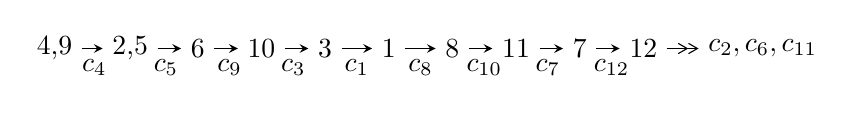
\begin{tikzpicture}[x=23pt, y=7pt]
	% node
	\node (A0) at (-1/8, 0) {4,9};
	\node (A1) at (17/16, 0) {2,5};
	\node (A2) at (17/8, 0) {6};
	\node (A3) at (25/8, 0) {10};
	\node (A4) at (33/8, 0) {3};
	\node (A5) at (41/8, 0) {1};
	\node (A6) at (49/8, 0) {8};
	\node (A7) at (57/8, 0) {11};
	\node (A8) at (65/8, 0) {7};
	\node (A9) at (73/8, 0) {12};
	\node (C1) at (1/2, -1) {$c_{4}$};
	\node (C2) at (13/8, -1) {$c_{5}$};
	\node (C3) at (21/8, -1) {$c_{9}$};
	\node (C4) at (29/8, -1) {$c_{3}$};
	\node (C5) at (37/8, -1) {$c_{1}$};
	\node (C6) at (45/8, -1) {$c_{8}$};
	\node (C7) at (53/8, -1) {$c_{10}$};
	\node (C8) at (61/8, -1) {$c_{7}$};
	\node (C9) at (69/8, -1) {$c_{12}$};
	\node (A10) at (11, 0) {$c_{2},c_{6},c_{11}$};

	% edge
	\draw[->,>=stealth]	
	(A0) edge (A1) (A1) edge (A2) (A2) edge (A3) (A3) edge (A4) (A4) edge (A5) (A5) edge (A6) (A6) edge (A7) (A7) edge (A8) (A8) edge (A9) ;
	\draw[->>,>={angle 60}]	
	(A9) edge (A10);
\end{tikzpicture} \\ 

\end{tabular} \\

\footnotetext{
The image of knot diagram is generated by the software ``\textbf{Draw programme}" developed by Andrew Bartholomew(\url{http://www.layer8.co.uk/maths/draw/index.htm\#Running-draw}), where we modified some parts for our purpose(\url{https://github.com/CATsTAILs/LinksPainter}).
}\phantom \\ \newline 
\centering \textbf{Ideals for irreducible components\footnotemark of $X_{\text{par}}$} 
 
\begin{align*}
I^u_{1}&=\langle 
- u^{23}-2 u^{22}+\cdots+b-1,\;u^{24}+3 u^{23}+\cdots+2 a+8 u,\;u^{25}+3 u^{24}+\cdots+8 u+2\rangle \\
I^u_{2}&=\langle 
2 u^{20} a-2 u^{20}+\cdots+b+1,\;-2 u^{20} a+2 u^{20}+\cdots-2 a+1,\;u^{21}- u^{20}+\cdots- u+1\rangle \\
I^u_{3}&=\langle 
b- u-1,\;2 a+u,\;u^2+2\rangle \\
\\
I^v_{1}&=\langle 
a,\;b+1,\;v+1\rangle \\
\end{align*}
\raggedright * 4 irreducible components of $\dim_{\mathbb{C}}=0$, with total 70 representations.\\
\footnotetext{All coefficients of polynomials are rational numbers. But the coefficients are sometimes approximated in decimal forms when there is not enough margin.}
\newpage
\renewcommand{\arraystretch}{1}
\centering \section*{I. $I^u_{1}= \langle - u^{23}-2 u^{22}+\cdots+b-1,\;u^{24}+3 u^{23}+\cdots+2 a+8 u,\;u^{25}+3 u^{24}+\cdots+8 u+2 \rangle$}
\flushleft \textbf{(i) Arc colorings}\\
\begin{tabular}{m{7pt} m{180pt} m{7pt} m{180pt} }
\flushright $a_{4}=$&$\begin{pmatrix}1\\0\end{pmatrix}$ \\
\flushright $a_{9}=$&$\begin{pmatrix}0\\u\end{pmatrix}$ \\
\flushright $a_{2}=$&$\begin{pmatrix}-\frac{1}{2} u^{24}-\frac{3}{2} u^{23}+\cdots-6 u^2-4 u\\u^{23}+2 u^{22}+\cdots+3 u+1\end{pmatrix}$ \\
\flushright $a_{5}=$&$\begin{pmatrix}1\\u^2\end{pmatrix}$ \\
\flushright $a_{6}=$&$\begin{pmatrix}-\frac{1}{2} u^{24}-\frac{1}{2} u^{23}+\cdots- u+1\\- u^{23}-2 u^{22}+\cdots-3 u-1\end{pmatrix}$ \\
\flushright $a_{10}=$&$\begin{pmatrix}- u\\u\end{pmatrix}$ \\
\flushright $a_{3}=$&$\begin{pmatrix}u^2+1\\- u^2\end{pmatrix}$ \\
\flushright $a_{1}=$&$\begin{pmatrix}-\frac{3}{2} u^{24}-\frac{9}{2} u^{23}+\cdots-14 u-3\\2 u^{23}+5 u^{22}+\cdots+9 u+3\end{pmatrix}$ \\
\flushright $a_{8}=$&$\begin{pmatrix}u\\u^3+u\end{pmatrix}$ \\
\flushright $a_{11}=$&$\begin{pmatrix}u^5+2 u^3- u\\u^7+3 u^5+2 u^3+u\end{pmatrix}$ \\
\flushright $a_{7}=$&$\begin{pmatrix}u^9+4 u^7+3 u^5-2 u^3+u\\u^{11}+5 u^9+8 u^7+5 u^5+3 u^3+u\end{pmatrix}$ \\
\flushright $a_{12}=$&$\begin{pmatrix}\frac{1}{2} u^{24}+\frac{3}{2} u^{23}+\cdots+3 u+1\\- u^{23}-2 u^{22}+\cdots-2 u-1\end{pmatrix}$\\&\end{tabular}
\flushleft \textbf{(ii) Obstruction class $= -1$}\\~\\
\flushleft \textbf{(iii) Cusp Shapes $= -8 u^{24}-18 u^{23}-126 u^{22}-242 u^{21}-840 u^{20}-1374 u^{19}-3088 u^{18}-4262 u^{17}-6822 u^{16}-7792 u^{15}-9236 u^{14}-8416 u^{13}-7450 u^{12}-5034 u^{11}-3220 u^{10}-1314 u^9-430 u^8+106 u^7+170 u^6+114 u^5-24 u^4-78 u^3-80 u^2-54 u-24$}\\~\\
\newpage\renewcommand{\arraystretch}{1}
\flushleft \textbf{(iv) u-Polynomials at the component}\newline \\
\begin{tabular}{m{50pt}|m{274pt}}
Crossings & \hspace{64pt}u-Polynomials at each crossing \\
\hline $$\begin{aligned}c_{1},c_{11}\end{aligned}$$&$\begin{aligned}
&u^{25}+13 u^{24}+\cdots+7 u+1
\end{aligned}$\\
\hline $$\begin{aligned}c_{2},c_{5},c_{6}\\c_{12}\end{aligned}$$&$\begin{aligned}
&u^{25}+u^{24}+\cdots+u+1
\end{aligned}$\\
\hline $$\begin{aligned}c_{3},c_{4},c_{8}\\c_{9}\end{aligned}$$&$\begin{aligned}
&u^{25}+3 u^{24}+\cdots+8 u+2
\end{aligned}$\\
\hline $$\begin{aligned}c_{7},c_{10}\end{aligned}$$&$\begin{aligned}
&u^{25}+3 u^{24}+\cdots-96 u^2+16
\end{aligned}$\\
\hline
\end{tabular}\\~\\
\newpage\renewcommand{\arraystretch}{1}
\flushleft \textbf{(v) Riley Polynomials at the component}\newline \\
\begin{tabular}{m{50pt}|m{274pt}}
Crossings & \hspace{64pt}Riley Polynomials at each crossing \\
\hline $$\begin{aligned}c_{1},c_{11}\end{aligned}$$&$\begin{aligned}
&y^{25}+3 y^{24}+\cdots+15 y-1
\end{aligned}$\\
\hline $$\begin{aligned}c_{2},c_{5},c_{6}\\c_{12}\end{aligned}$$&$\begin{aligned}
&y^{25}-13 y^{24}+\cdots+7 y-1
\end{aligned}$\\
\hline $$\begin{aligned}c_{3},c_{4},c_{8}\\c_{9}\end{aligned}$$&$\begin{aligned}
&y^{25}+27 y^{24}+\cdots+8 y-4
\end{aligned}$\\
\hline $$\begin{aligned}c_{7},c_{10}\end{aligned}$$&$\begin{aligned}
&y^{25}+19 y^{24}+\cdots+3072 y-256
\end{aligned}$\\
\hline
\end{tabular}\\~\\
\newpage\flushleft \textbf{(vi) Complex Volumes and Cusp Shapes}
$$\begin{array}{c|c|c}  
\text{Solutions to }I^u_{1}& \I (\text{vol} + \sqrt{-1}CS) & \text{Cusp shape}\\
 \hline 
\begin{aligned}
u &= -0.651480 + 0.569397 I \\
a &= -1.31726 - 1.62418 I \\
b &= -0.115293 + 0.307631 I\end{aligned}
 & -8.03966 + 11.38840 I & -12.3901 - 9.1803 I \\ \hline\begin{aligned}
u &= -0.651480 - 0.569397 I \\
a &= -1.31726 + 1.62418 I \\
b &= -0.115293 - 0.307631 I\end{aligned}
 & -8.03966 - 11.38840 I & -12.3901 + 9.1803 I \\ \hline\begin{aligned}
u &= -0.683025 + 0.436288 I \\
a &= \phantom{-}0.878062 + 0.233968 I \\
b &= -0.828869 - 0.938936 I\end{aligned}
 & -8.43694 - 6.90173 I & -13.44025 + 3.63036 I \\ \hline\begin{aligned}
u &= -0.683025 - 0.436288 I \\
a &= \phantom{-}0.878062 - 0.233968 I \\
b &= -0.828869 + 0.938936 I\end{aligned}
 & -8.43694 + 6.90173 I & -13.44025 - 3.63036 I \\ \hline\begin{aligned}
u &= \phantom{-}0.412040 + 0.685850 I \\
a &= -0.47621 + 1.83448 I \\
b &= \phantom{-}0.072745 - 0.306443 I\end{aligned}
 & -0.17864 - 6.77079 I & -7.18283 + 10.35931 I \\ \hline\begin{aligned}
u &= \phantom{-}0.412040 - 0.685850 I \\
a &= -0.47621 - 1.83448 I \\
b &= \phantom{-}0.072745 + 0.306443 I\end{aligned}
 & -0.17864 + 6.77079 I & -7.18283 - 10.35931 I \\ \hline\begin{aligned}
u &= -0.558289 + 0.498098 I \\
a &= \phantom{-}0.708276 + 0.173203 I \\
b &= \phantom{-}0.206889 + 0.374837 I\end{aligned}
 & -1.41690 + 1.92070 I & -6.23376 - 3.47212 I \\ \hline\begin{aligned}
u &= -0.558289 - 0.498098 I \\
a &= \phantom{-}0.708276 - 0.173203 I \\
b &= \phantom{-}0.206889 - 0.374837 I\end{aligned}
 & -1.41690 - 1.92070 I & -6.23376 + 3.47212 I \\ \hline\begin{aligned}
u &= \phantom{-}0.023881 + 0.737446 I \\
a &= \phantom{-}0.622644 - 0.953292 I \\
b &= \phantom{-}0.315147 + 0.069716 I\end{aligned}
 & \phantom{-}1.88598 + 1.45733 I & -1.26812 - 4.21250 I \\ \hline\begin{aligned}
u &= \phantom{-}0.023881 - 0.737446 I \\
a &= \phantom{-}0.622644 + 0.953292 I \\
b &= \phantom{-}0.315147 - 0.069716 I\end{aligned}
 & \phantom{-}1.88598 - 1.45733 I & -1.26812 + 4.21250 I\\
 \hline 
 \end{array}$$\newpage$$\begin{array}{c|c|c}  
\text{Solutions to }I^u_{1}& \I (\text{vol} + \sqrt{-1}CS) & \text{Cusp shape}\\
 \hline 
\begin{aligned}
u &= \phantom{-}0.054153 + 1.332330 I \\
a &= -0.077174 - 0.173973 I \\
b &= \phantom{-}0.971993 + 0.051958 I\end{aligned}
 & \phantom{-}2.62061 + 1.17903 I & -5.07770 - 5.84448 I \\ \hline\begin{aligned}
u &= \phantom{-}0.054153 - 1.332330 I \\
a &= -0.077174 + 0.173973 I \\
b &= \phantom{-}0.971993 - 0.051958 I\end{aligned}
 & \phantom{-}2.62061 - 1.17903 I & -5.07770 + 5.84448 I \\ \hline\begin{aligned}
u &= \phantom{-}0.573959 + 0.177466 I \\
a &= \phantom{-}0.874794 - 0.104864 I \\
b &= -0.619515 + 0.565743 I\end{aligned}
 & -1.76413 + 3.37976 I & -11.30285 - 5.40492 I \\ \hline\begin{aligned}
u &= \phantom{-}0.573959 - 0.177466 I \\
a &= \phantom{-}0.874794 + 0.104864 I \\
b &= -0.619515 - 0.565743 I\end{aligned}
 & -1.76413 - 3.37976 I & -11.30285 + 5.40492 I \\ \hline\begin{aligned}
u &= -0.21436 + 1.46119 I \\
a &= \phantom{-}0.144093 + 0.127422 I \\
b &= \phantom{-}0.970978 + 0.088622 I\end{aligned}
 & -2.31754 - 3.68038 I & -10.19471 + 3.82630 I \\ \hline\begin{aligned}
u &= -0.21436 - 1.46119 I \\
a &= \phantom{-}0.144093 - 0.127422 I \\
b &= \phantom{-}0.970978 - 0.088622 I\end{aligned}
 & -2.31754 + 3.68038 I & -10.19471 - 3.82630 I \\ \hline\begin{aligned}
u &= -0.16059 + 1.52773 I \\
a &= -0.753431 - 0.916816 I \\
b &= \phantom{-}1.12967 + 1.67442 I\end{aligned}
 & \phantom{-}5.30944 + 4.47743 I & -2.55629 - 2.34174 I \\ \hline\begin{aligned}
u &= -0.16059 - 1.52773 I \\
a &= -0.753431 + 0.916816 I \\
b &= \phantom{-}1.12967 - 1.67442 I\end{aligned}
 & \phantom{-}5.30944 - 4.47743 I & -2.55629 + 2.34174 I \\ \hline\begin{aligned}
u &= -0.20643 + 1.54713 I \\
a &= \phantom{-}0.25239 + 1.93004 I \\
b &= -0.58907 - 4.16682 I\end{aligned}
 & -1.0459 + 14.5269 I & -8.91507 - 8.56336 I \\ \hline\begin{aligned}
u &= -0.20643 - 1.54713 I \\
a &= \phantom{-}0.25239 - 1.93004 I \\
b &= -0.58907 + 4.16682 I\end{aligned}
 & -1.0459 - 14.5269 I & -8.91507 + 8.56336 I\\
 \hline 
 \end{array}$$\newpage$$\begin{array}{c|c|c}  
\text{Solutions to }I^u_{1}& \I (\text{vol} + \sqrt{-1}CS) & \text{Cusp shape}\\
 \hline 
\begin{aligned}
u &= \phantom{-}0.01772 + 1.57526 I \\
a &= -0.91307 + 1.41013 I \\
b &= \phantom{-}1.55989 - 2.89337 I\end{aligned}
 & \phantom{-}9.63847 + 1.22771 I & -0.35980 - 3.25847 I \\ \hline\begin{aligned}
u &= \phantom{-}0.01772 - 1.57526 I \\
a &= -0.91307 - 1.41013 I \\
b &= \phantom{-}1.55989 + 2.89337 I\end{aligned}
 & \phantom{-}9.63847 - 1.22771 I & -0.35980 + 3.25847 I \\ \hline\begin{aligned}
u &= \phantom{-}0.10120 + 1.57793 I \\
a &= -0.39162 - 1.95619 I \\
b &= \phantom{-}0.60654 + 4.12616 I\end{aligned}
 & \phantom{-}7.45823 - 8.58001 I & -4.35516 + 8.14193 I \\ \hline\begin{aligned}
u &= \phantom{-}0.10120 - 1.57793 I \\
a &= -0.39162 + 1.95619 I \\
b &= \phantom{-}0.60654 - 4.12616 I\end{aligned}
 & \phantom{-}7.45823 + 8.58001 I & -4.35516 - 8.14193 I \\ \hline\begin{aligned}
u &= -0.417568\phantom{ +0.000000I} \\
a &= \phantom{-}0.897008\phantom{ +0.000000I} \\
b &= -0.362213\phantom{ +0.000000I}\end{aligned}
 & -0.846371\phantom{ +0.000000I} & -11.4470\phantom{ +0.000000I}\\
 \hline 
 \end{array}$$\newpage\newpage\renewcommand{\arraystretch}{1}
\centering \section*{II. $I^u_{2}= \langle 2 u^{20} a-2 u^{20}+\cdots+b+1,\;-2 u^{20} a+2 u^{20}+\cdots-2 a+1,\;u^{21}- u^{20}+\cdots- u+1 \rangle$}
\flushleft \textbf{(i) Arc colorings}\\
\begin{tabular}{m{7pt} m{180pt} m{7pt} m{180pt} }
\flushright $a_{4}=$&$\begin{pmatrix}1\\0\end{pmatrix}$ \\
\flushright $a_{9}=$&$\begin{pmatrix}0\\u\end{pmatrix}$ \\
\flushright $a_{2}=$&$\begin{pmatrix}a\\-2 u^{20} a+2 u^{20}+\cdots-3 u-1\end{pmatrix}$ \\
\flushright $a_{5}=$&$\begin{pmatrix}1\\u^2\end{pmatrix}$ \\
\flushright $a_{6}=$&$\begin{pmatrix}-2 u^{20} a+2 u^{20}+\cdots+a-1\\2 u^{20} a-2 u^{20}+\cdots+3 u+1\end{pmatrix}$ \\
\flushright $a_{10}=$&$\begin{pmatrix}- u\\u\end{pmatrix}$ \\
\flushright $a_{3}=$&$\begin{pmatrix}u^2+1\\- u^2\end{pmatrix}$ \\
\flushright $a_{1}=$&$\begin{pmatrix}-2 u^{20} a+2 u^{20}+\cdots+a-1\\-2 u^{20} a+2 u^{20}+\cdots- u-1\end{pmatrix}$ \\
\flushright $a_{8}=$&$\begin{pmatrix}u\\u^3+u\end{pmatrix}$ \\
\flushright $a_{11}=$&$\begin{pmatrix}u^5+2 u^3- u\\u^7+3 u^5+2 u^3+u\end{pmatrix}$ \\
\flushright $a_{7}=$&$\begin{pmatrix}u^9+4 u^7+3 u^5-2 u^3+u\\u^{11}+5 u^9+8 u^7+5 u^5+3 u^3+u\end{pmatrix}$ \\
\flushright $a_{12}=$&$\begin{pmatrix}-2 u^{20} a+2 u^{20}+\cdots+a-1\\- u^{17} a-9 u^{15} a+\cdots+2 u-1\end{pmatrix}$\\&\end{tabular}
\flushleft \textbf{(ii) Obstruction class $= -1$}\\~\\
\flushleft \textbf{(iii) Cusp Shapes $= 4 u^{20}-4 u^{19}+48 u^{18}-40 u^{17}+232 u^{16}-156 u^{15}+572 u^{14}-292 u^{13}+756 u^{12}-256 u^{11}+552 u^{10}-88 u^9+316 u^8-24 u^7+204 u^6-8 u^5+48 u^4+20 u^3+16 u^2+16 u-10$}\\~\\
\newpage\renewcommand{\arraystretch}{1}
\flushleft \textbf{(iv) u-Polynomials at the component}\newline \\
\begin{tabular}{m{50pt}|m{274pt}}
Crossings & \hspace{64pt}u-Polynomials at each crossing \\
\hline $$\begin{aligned}c_{1},c_{11}\end{aligned}$$&$\begin{aligned}
&u^{42}+25 u^{41}+\cdots+52 u+9
\end{aligned}$\\
\hline $$\begin{aligned}c_{2},c_{5},c_{6}\\c_{12}\end{aligned}$$&$\begin{aligned}
&u^{42}+u^{41}+\cdots+8 u+3
\end{aligned}$\\
\hline $$\begin{aligned}c_{3},c_{4},c_{8}\\c_{9}\end{aligned}$$&$\begin{aligned}
&(u^{21}- u^{20}+\cdots- u+1)^{2}
\end{aligned}$\\
\hline $$\begin{aligned}c_{7},c_{10}\end{aligned}$$&$\begin{aligned}
&(u^{21}+3 u^{20}+\cdots+5 u+3)^{2}
\end{aligned}$\\
\hline
\end{tabular}\\~\\
\newpage\renewcommand{\arraystretch}{1}
\flushleft \textbf{(v) Riley Polynomials at the component}\newline \\
\begin{tabular}{m{50pt}|m{274pt}}
Crossings & \hspace{64pt}Riley Polynomials at each crossing \\
\hline $$\begin{aligned}c_{1},c_{11}\end{aligned}$$&$\begin{aligned}
&y^{42}-17 y^{41}+\cdots-868 y+81
\end{aligned}$\\
\hline $$\begin{aligned}c_{2},c_{5},c_{6}\\c_{12}\end{aligned}$$&$\begin{aligned}
&y^{42}-25 y^{41}+\cdots-52 y+9
\end{aligned}$\\
\hline $$\begin{aligned}c_{3},c_{4},c_{8}\\c_{9}\end{aligned}$$&$\begin{aligned}
&(y^{21}+23 y^{20}+\cdots-5 y-1)^{2}
\end{aligned}$\\
\hline $$\begin{aligned}c_{7},c_{10}\end{aligned}$$&$\begin{aligned}
&(y^{21}+19 y^{20}+\cdots+7 y-9)^{2}
\end{aligned}$\\
\hline
\end{tabular}\\~\\
\newpage\flushleft \textbf{(vi) Complex Volumes and Cusp Shapes}
$$\begin{array}{c|c|c}  
\text{Solutions to }I^u_{2}& \I (\text{vol} + \sqrt{-1}CS) & \text{Cusp shape}\\
 \hline 
\begin{aligned}
u &= \phantom{-}0.613284 + 0.552606 I \\
a &= \phantom{-}0.663670 - 0.167306 I \\
b &= \phantom{-}0.258836 - 0.415847 I\end{aligned}
 & -4.68217 - 6.45770 I & -9.45356 + 6.39068 I \\ \hline\begin{aligned}
u &= \phantom{-}0.613284 + 0.552606 I \\
a &= -1.31427 + 1.76259 I \\
b &= -0.095105 - 0.288417 I\end{aligned}
 & -4.68217 - 6.45770 I & -9.45356 + 6.39068 I \\ \hline\begin{aligned}
u &= \phantom{-}0.613284 - 0.552606 I \\
a &= \phantom{-}0.663670 + 0.167306 I \\
b &= \phantom{-}0.258836 + 0.415847 I\end{aligned}
 & -4.68217 + 6.45770 I & -9.45356 - 6.39068 I \\ \hline\begin{aligned}
u &= \phantom{-}0.613284 - 0.552606 I \\
a &= -1.31427 - 1.76259 I \\
b &= -0.095105 + 0.288417 I\end{aligned}
 & -4.68217 + 6.45770 I & -9.45356 - 6.39068 I \\ \hline\begin{aligned}
u &= -0.621912 + 0.497822 I \\
a &= \phantom{-}0.918873 + 0.252143 I \\
b &= -0.963307 - 0.936491 I\end{aligned}
 & -8.79207 + 2.11040 I & -13.9124 - 3.3898 I \\ \hline\begin{aligned}
u &= -0.621912 + 0.497822 I \\
a &= -1.51743 - 1.81016 I \\
b &= -0.112550 + 0.257173 I\end{aligned}
 & -8.79207 + 2.11040 I & -13.9124 - 3.3898 I \\ \hline\begin{aligned}
u &= -0.621912 - 0.497822 I \\
a &= \phantom{-}0.918873 - 0.252143 I \\
b &= -0.963307 + 0.936491 I\end{aligned}
 & -8.79207 - 2.11040 I & -13.9124 + 3.3898 I \\ \hline\begin{aligned}
u &= -0.621912 - 0.497822 I \\
a &= -1.51743 + 1.81016 I \\
b &= -0.112550 - 0.257173 I\end{aligned}
 & -8.79207 - 2.11040 I & -13.9124 + 3.3898 I \\ \hline\begin{aligned}
u &= \phantom{-}0.630060 + 0.435502 I \\
a &= \phantom{-}0.902520 - 0.223812 I \\
b &= -0.882881 + 0.878598 I\end{aligned}
 & -5.02710 + 2.23968 I & -10.49766 - 0.17506 I \\ \hline\begin{aligned}
u &= \phantom{-}0.630060 + 0.435502 I \\
a &= \phantom{-}0.706600 - 0.119856 I \\
b &= \phantom{-}0.159229 - 0.443860 I\end{aligned}
 & -5.02710 + 2.23968 I & -10.49766 - 0.17506 I\\
 \hline 
 \end{array}$$\newpage$$\begin{array}{c|c|c}  
\text{Solutions to }I^u_{2}& \I (\text{vol} + \sqrt{-1}CS) & \text{Cusp shape}\\
 \hline 
\begin{aligned}
u &= \phantom{-}0.630060 - 0.435502 I \\
a &= \phantom{-}0.902520 + 0.223812 I \\
b &= -0.882881 - 0.878598 I\end{aligned}
 & -5.02710 - 2.23968 I & -10.49766 + 0.17506 I \\ \hline\begin{aligned}
u &= \phantom{-}0.630060 - 0.435502 I \\
a &= \phantom{-}0.706600 + 0.119856 I \\
b &= \phantom{-}0.159229 + 0.443860 I\end{aligned}
 & -5.02710 - 2.23968 I & -10.49766 + 0.17506 I \\ \hline\begin{aligned}
u &= -0.264535 + 0.686798 I \\
a &= \phantom{-}0.696463 + 0.484067 I \\
b &= \phantom{-}0.329117 + 0.122623 I\end{aligned}
 & \phantom{-}1.27822 + 2.45481 I & -3.17392 - 5.13736 I \\ \hline\begin{aligned}
u &= -0.264535 + 0.686798 I \\
a &= \phantom{-}0.08311 - 1.80534 I \\
b &= \phantom{-}0.158741 + 0.236037 I\end{aligned}
 & \phantom{-}1.27822 + 2.45481 I & -3.17392 - 5.13736 I \\ \hline\begin{aligned}
u &= -0.264535 - 0.686798 I \\
a &= \phantom{-}0.696463 - 0.484067 I \\
b &= \phantom{-}0.329117 - 0.122623 I\end{aligned}
 & \phantom{-}1.27822 - 2.45481 I & -3.17392 + 5.13736 I \\ \hline\begin{aligned}
u &= -0.264535 - 0.686798 I \\
a &= \phantom{-}0.08311 + 1.80534 I \\
b &= \phantom{-}0.158741 - 0.236037 I\end{aligned}
 & \phantom{-}1.27822 - 2.45481 I & -3.17392 + 5.13736 I \\ \hline\begin{aligned}
u &= \phantom{-}0.17161 + 1.47674 I \\
a &= -0.734220 + 0.822924 I \\
b &= \phantom{-}1.13685 - 1.39375 I\end{aligned}
 & \phantom{-}1.167780 - 0.589478 I & -6.95446 - 0.27365 I \\ \hline\begin{aligned}
u &= \phantom{-}0.17161 + 1.47674 I \\
a &= \phantom{-}0.126348 - 0.107181 I \\
b &= \phantom{-}0.987004 - 0.067695 I\end{aligned}
 & \phantom{-}1.167780 - 0.589478 I & -6.95446 - 0.27365 I \\ \hline\begin{aligned}
u &= \phantom{-}0.17161 - 1.47674 I \\
a &= -0.734220 - 0.822924 I \\
b &= \phantom{-}1.13685 + 1.39375 I\end{aligned}
 & \phantom{-}1.167780 + 0.589478 I & -6.95446 + 0.27365 I \\ \hline\begin{aligned}
u &= \phantom{-}0.17161 - 1.47674 I \\
a &= \phantom{-}0.126348 + 0.107181 I \\
b &= \phantom{-}0.987004 + 0.067695 I\end{aligned}
 & \phantom{-}1.167780 + 0.589478 I & -6.95446 + 0.27365 I\\
 \hline 
 \end{array}$$\newpage$$\begin{array}{c|c|c}  
\text{Solutions to }I^u_{2}& \I (\text{vol} + \sqrt{-1}CS) & \text{Cusp shape}\\
 \hline 
\begin{aligned}
u &= \phantom{-}0.03893 + 1.51037 I \\
a &= \phantom{-}0.0956698 - 0.0258264 I \\
b &= \phantom{-}1.020350 - 0.014142 I\end{aligned}
 & \phantom{-}3.29266 - 1.66521 I & -6.44233 + 3.90994 I \\ \hline\begin{aligned}
u &= \phantom{-}0.03893 + 1.51037 I \\
a &= -1.43429 - 2.27893 I \\
b &= \phantom{-}2.73302 + 4.65122 I\end{aligned}
 & \phantom{-}3.29266 - 1.66521 I & -6.44233 + 3.90994 I \\ \hline\begin{aligned}
u &= \phantom{-}0.03893 - 1.51037 I \\
a &= \phantom{-}0.0956698 + 0.0258264 I \\
b &= \phantom{-}1.020350 + 0.014142 I\end{aligned}
 & \phantom{-}3.29266 + 1.66521 I & -6.44233 - 3.90994 I \\ \hline\begin{aligned}
u &= \phantom{-}0.03893 - 1.51037 I \\
a &= -1.43429 + 2.27893 I \\
b &= \phantom{-}2.73302 - 4.65122 I\end{aligned}
 & \phantom{-}3.29266 + 1.66521 I & -6.44233 - 3.90994 I \\ \hline\begin{aligned}
u &= -0.18541 + 1.51409 I \\
a &= \phantom{-}0.144635 + 0.094757 I \\
b &= \phantom{-}1.004590 + 0.080707 I\end{aligned}
 & -2.18398 + 5.00460 I & -10.15348 - 3.34739 I \\ \hline\begin{aligned}
u &= -0.18541 + 1.51409 I \\
a &= \phantom{-}0.31289 + 2.15828 I \\
b &= -0.68662 - 4.58559 I\end{aligned}
 & -2.18398 + 5.00460 I & -10.15348 - 3.34739 I \\ \hline\begin{aligned}
u &= -0.18541 - 1.51409 I \\
a &= \phantom{-}0.144635 - 0.094757 I \\
b &= \phantom{-}1.004590 - 0.080707 I\end{aligned}
 & -2.18398 - 5.00460 I & -10.15348 + 3.34739 I \\ \hline\begin{aligned}
u &= -0.18541 - 1.51409 I \\
a &= \phantom{-}0.31289 - 2.15828 I \\
b &= -0.68662 + 4.58559 I\end{aligned}
 & -2.18398 - 5.00460 I & -10.15348 + 3.34739 I \\ \hline\begin{aligned}
u &= \phantom{-}0.224591 + 0.416086 I \\
a &= \phantom{-}1.057800 - 0.095161 I \\
b &= -1.241430 + 0.325944 I\end{aligned}
 & -3.19863 - 0.86446 I & -9.82793 + 8.05526 I \\ \hline\begin{aligned}
u &= \phantom{-}0.224591 + 0.416086 I \\
a &= \phantom{-}0.94469 + 4.04424 I \\
b &= \phantom{-}0.0521710 - 0.1030170 I\end{aligned}
 & -3.19863 - 0.86446 I & -9.82793 + 8.05526 I\\
 \hline 
 \end{array}$$\newpage$$\begin{array}{c|c|c}  
\text{Solutions to }I^u_{2}& \I (\text{vol} + \sqrt{-1}CS) & \text{Cusp shape}\\
 \hline 
\begin{aligned}
u &= \phantom{-}0.224591 - 0.416086 I \\
a &= \phantom{-}1.057800 + 0.095161 I \\
b &= -1.241430 - 0.325944 I\end{aligned}
 & -3.19863 + 0.86446 I & -9.82793 - 8.05526 I \\ \hline\begin{aligned}
u &= \phantom{-}0.224591 - 0.416086 I \\
a &= \phantom{-}0.94469 - 4.04424 I \\
b &= \phantom{-}0.0521710 + 0.1030170 I\end{aligned}
 & -3.19863 + 0.86446 I & -9.82793 - 8.05526 I \\ \hline\begin{aligned}
u &= -0.463882\phantom{ +0.000000I} \\
a &= \phantom{-}0.882798 + 0.014771 I \\
b &= -0.402171 - 0.224592 I\end{aligned}
 & -0.823381\phantom{ +0.000000I} & -10.2590\phantom{ +0.000000I} \\ \hline\begin{aligned}
u &= -0.463882\phantom{ +0.000000I} \\
a &= \phantom{-}0.882798 - 0.014771 I \\
b &= -0.402171 + 0.224592 I\end{aligned}
 & -0.823381\phantom{ +0.000000I} & -10.2590\phantom{ +0.000000I} \\ \hline\begin{aligned}
u &= \phantom{-}0.18830 + 1.54115 I \\
a &= -0.703578 + 0.924146 I \\
b &= \phantom{-}0.97403 - 1.67776 I\end{aligned}
 & \phantom{-}2.24917 - 9.37044 I & -5.88057 + 5.65030 I \\ \hline\begin{aligned}
u &= \phantom{-}0.18830 + 1.54115 I \\
a &= \phantom{-}0.20144 - 2.02236 I \\
b &= -0.49031 + 4.33008 I\end{aligned}
 & \phantom{-}2.24917 - 9.37044 I & -5.88057 + 5.65030 I \\ \hline\begin{aligned}
u &= \phantom{-}0.18830 - 1.54115 I \\
a &= -0.703578 - 0.924146 I \\
b &= \phantom{-}0.97403 + 1.67776 I\end{aligned}
 & \phantom{-}2.24917 + 9.37044 I & -5.88057 - 5.65030 I \\ \hline\begin{aligned}
u &= \phantom{-}0.18830 - 1.54115 I \\
a &= \phantom{-}0.20144 + 2.02236 I \\
b &= -0.49031 - 4.33008 I\end{aligned}
 & \phantom{-}2.24917 + 9.37044 I & -5.88057 - 5.65030 I \\ \hline\begin{aligned}
u &= -0.06297 + 1.57333 I \\
a &= -0.87578 - 1.19347 I \\
b &= \phantom{-}1.44224 + 2.40342 I\end{aligned}
 & \phantom{-}8.90560 + 3.59224 I & -1.57394 - 3.20950 I \\ \hline\begin{aligned}
u &= -0.06297 + 1.57333 I \\
a &= -0.65794 + 1.88952 I \\
b &= \phantom{-}1.11820 - 3.94658 I\end{aligned}
 & \phantom{-}8.90560 + 3.59224 I & -1.57394 - 3.20950 I\\
 \hline 
 \end{array}$$\newpage$$\begin{array}{c|c|c}  
\text{Solutions to }I^u_{2}& \I (\text{vol} + \sqrt{-1}CS) & \text{Cusp shape}\\
 \hline 
\begin{aligned}
u &= -0.06297 - 1.57333 I \\
a &= -0.87578 + 1.19347 I \\
b &= \phantom{-}1.44224 - 2.40342 I\end{aligned}
 & \phantom{-}8.90560 - 3.59224 I & -1.57394 + 3.20950 I \\ \hline\begin{aligned}
u &= -0.06297 - 1.57333 I \\
a &= -0.65794 - 1.88952 I \\
b &= \phantom{-}1.11820 + 3.94658 I\end{aligned}
 & \phantom{-}8.90560 - 3.59224 I & -1.57394 + 3.20950 I\\
 \hline 
 \end{array}$$\newpage\newpage\renewcommand{\arraystretch}{1}
\centering \section*{III. $I^u_{3}= \langle b- u-1,\;2 a+u,\;u^2+2 \rangle$}
\flushleft \textbf{(i) Arc colorings}\\
\begin{tabular}{m{7pt} m{180pt} m{7pt} m{180pt} }
\flushright $a_{4}=$&$\begin{pmatrix}1\\0\end{pmatrix}$ \\
\flushright $a_{9}=$&$\begin{pmatrix}0\\u\end{pmatrix}$ \\
\flushright $a_{2}=$&$\begin{pmatrix}-\frac{1}{2} u\\u+1\end{pmatrix}$ \\
\flushright $a_{5}=$&$\begin{pmatrix}1\\-2\end{pmatrix}$ \\
\flushright $a_{6}=$&$\begin{pmatrix}-\frac{1}{2} u+1\\u-1\end{pmatrix}$ \\
\flushright $a_{10}=$&$\begin{pmatrix}- u\\u\end{pmatrix}$ \\
\flushright $a_{3}=$&$\begin{pmatrix}-1\\2\end{pmatrix}$ \\
\flushright $a_{1}=$&$\begin{pmatrix}-\frac{1}{2} u+1\\u-1\end{pmatrix}$ \\
\flushright $a_{8}=$&$\begin{pmatrix}u\\- u\end{pmatrix}$ \\
\flushright $a_{11}=$&$\begin{pmatrix}- u\\u\end{pmatrix}$ \\
\flushright $a_{7}=$&$\begin{pmatrix}u\\- u\end{pmatrix}$ \\
\flushright $a_{12}=$&$\begin{pmatrix}-\frac{3}{2} u+1\\2 u-1\end{pmatrix}$\\&\end{tabular}
\flushleft \textbf{(ii) Obstruction class $= 1$}\\~\\
\flushleft \textbf{(iii) Cusp Shapes $= -12$}\\~\\
\newpage\renewcommand{\arraystretch}{1}
\flushleft \textbf{(iv) u-Polynomials at the component}\newline \\
\begin{tabular}{m{50pt}|m{274pt}}
Crossings & \hspace{64pt}u-Polynomials at each crossing \\
\hline $$\begin{aligned}c_{1},c_{5},c_{11}\\c_{12}\end{aligned}$$&$\begin{aligned}
&(u-1)^2
\end{aligned}$\\
\hline $$\begin{aligned}c_{2},c_{6}\end{aligned}$$&$\begin{aligned}
&(u+1)^2
\end{aligned}$\\
\hline $$\begin{aligned}c_{3},c_{4},c_{8}\\c_{9}\end{aligned}$$&$\begin{aligned}
&u^2+2
\end{aligned}$\\
\hline $$\begin{aligned}c_{7},c_{10}\end{aligned}$$&$\begin{aligned}
&u^2
\end{aligned}$\\
\hline
\end{tabular}\\~\\
\newpage\renewcommand{\arraystretch}{1}
\flushleft \textbf{(v) Riley Polynomials at the component}\newline \\
\begin{tabular}{m{50pt}|m{274pt}}
Crossings & \hspace{64pt}Riley Polynomials at each crossing \\
\hline $$\begin{aligned}c_{1},c_{2},c_{5}\\c_{6},c_{11},c_{12}\end{aligned}$$&$\begin{aligned}
&(y-1)^2
\end{aligned}$\\
\hline $$\begin{aligned}c_{3},c_{4},c_{8}\\c_{9}\end{aligned}$$&$\begin{aligned}
&(y+2)^2
\end{aligned}$\\
\hline $$\begin{aligned}c_{7},c_{10}\end{aligned}$$&$\begin{aligned}
&y^2
\end{aligned}$\\
\hline
\end{tabular}\\~\\
\newpage\flushleft \textbf{(vi) Complex Volumes and Cusp Shapes}
$$\begin{array}{c|c|c}  
\text{Solutions to }I^u_{3}& \I (\text{vol} + \sqrt{-1}CS) & \text{Cusp shape}\\
 \hline 
\begin{aligned}
u &= \phantom{-0.000000 -}1.414210 I \\
a &= \phantom{-0.000000 } -0.707107 I \\
b &= \phantom{-}1.00000 + 1.41421 I\end{aligned}
 & \phantom{-}1.64493\phantom{ +0.000000I} & -12.0000\phantom{ +0.000000I} \\ \hline\begin{aligned}
u &= \phantom{-0.000000 } -1.414210 I \\
a &= \phantom{-0.000000 -}0.707107 I \\
b &= \phantom{-}1.00000 - 1.41421 I\end{aligned}
 & \phantom{-}1.64493\phantom{ +0.000000I} & -12.0000\phantom{ +0.000000I}\\
 \hline 
 \end{array}$$\newpage\newpage\renewcommand{\arraystretch}{1}
\centering \section*{IV. $I^v_{1}= \langle a,\;b+1,\;v+1 \rangle$}
\flushleft \textbf{(i) Arc colorings}\\
\begin{tabular}{m{7pt} m{180pt} m{7pt} m{180pt} }
\flushright $a_{4}=$&$\begin{pmatrix}1\\0\end{pmatrix}$ \\
\flushright $a_{9}=$&$\begin{pmatrix}-1\\0\end{pmatrix}$ \\
\flushright $a_{2}=$&$\begin{pmatrix}0\\-1\end{pmatrix}$ \\
\flushright $a_{5}=$&$\begin{pmatrix}1\\0\end{pmatrix}$ \\
\flushright $a_{6}=$&$\begin{pmatrix}1\\1\end{pmatrix}$ \\
\flushright $a_{10}=$&$\begin{pmatrix}-1\\0\end{pmatrix}$ \\
\flushright $a_{3}=$&$\begin{pmatrix}1\\0\end{pmatrix}$ \\
\flushright $a_{1}=$&$\begin{pmatrix}-1\\-1\end{pmatrix}$ \\
\flushright $a_{8}=$&$\begin{pmatrix}-1\\0\end{pmatrix}$ \\
\flushright $a_{11}=$&$\begin{pmatrix}-1\\0\end{pmatrix}$ \\
\flushright $a_{7}=$&$\begin{pmatrix}-1\\0\end{pmatrix}$ \\
\flushright $a_{12}=$&$\begin{pmatrix}-2\\-1\end{pmatrix}$\\&\end{tabular}
\flushleft \textbf{(ii) Obstruction class $= 1$}\\~\\
\flushleft \textbf{(iii) Cusp Shapes $= -12$}\\~\\
\newpage\renewcommand{\arraystretch}{1}
\flushleft \textbf{(iv) u-Polynomials at the component}\newline \\
\begin{tabular}{m{50pt}|m{274pt}}
Crossings & \hspace{64pt}u-Polynomials at each crossing \\
\hline $$\begin{aligned}c_{1},c_{2},c_{6}\\c_{11}\end{aligned}$$&$\begin{aligned}
&u-1
\end{aligned}$\\
\hline $$\begin{aligned}c_{3},c_{4},c_{7}\\c_{8},c_{9},c_{10}\end{aligned}$$&$\begin{aligned}
&u
\end{aligned}$\\
\hline $$\begin{aligned}c_{5},c_{12}\end{aligned}$$&$\begin{aligned}
&u+1
\end{aligned}$\\
\hline
\end{tabular}\\~\\
\newpage\renewcommand{\arraystretch}{1}
\flushleft \textbf{(v) Riley Polynomials at the component}\newline \\
\begin{tabular}{m{50pt}|m{274pt}}
Crossings & \hspace{64pt}Riley Polynomials at each crossing \\
\hline $$\begin{aligned}c_{1},c_{2},c_{5}\\c_{6},c_{11},c_{12}\end{aligned}$$&$\begin{aligned}
&y-1
\end{aligned}$\\
\hline $$\begin{aligned}c_{3},c_{4},c_{7}\\c_{8},c_{9},c_{10}\end{aligned}$$&$\begin{aligned}
&y
\end{aligned}$\\
\hline
\end{tabular}\\~\\
\newpage\flushleft \textbf{(vi) Complex Volumes and Cusp Shapes}
$$\begin{array}{c|c|c}  
\text{Solutions to }I^v_{1}& \I (\text{vol} + \sqrt{-1}CS) & \text{Cusp shape}\\
 \hline 
\begin{aligned}
v &= -1.00000\phantom{ +0.000000I} \\
a &= \phantom{-0.000000 } 0 \\
b &= -1.00000\phantom{ +0.000000I}\end{aligned}
 & -3.28987\phantom{ +0.000000I} & -12.0000\phantom{ +0.000000I}\\
 \hline 
 \end{array}$$\newpage
\newpage\renewcommand{\arraystretch}{1}
\centering \section*{ V. u-Polynomials}
\begin{tabular}{m{50pt}|m{274pt}}
Crossings & \hspace{64pt}u-Polynomials at each crossing \\
\hline $$\begin{aligned}c_{1},c_{11}\end{aligned}$$&$\begin{aligned}
&((u-1)^3)(u^{25}+13 u^{24}+\cdots+7 u+1)(u^{42}+25 u^{41}+\cdots+52 u+9)
\end{aligned}$\\
\hline $$\begin{aligned}c_{2},c_{6}\end{aligned}$$&$\begin{aligned}
&(u-1)(u+1)^2(u^{25}+u^{24}+\cdots+u+1)(u^{42}+u^{41}+\cdots+8 u+3)
\end{aligned}$\\
\hline $$\begin{aligned}c_{3},c_{4},c_{8}\\c_{9}\end{aligned}$$&$\begin{aligned}
&u(u^2+2)(u^{21}- u^{20}+\cdots- u+1)^{2}(u^{25}+3 u^{24}+\cdots+8 u+2)
\end{aligned}$\\
\hline $$\begin{aligned}c_{5},c_{12}\end{aligned}$$&$\begin{aligned}
&((u-1)^2)(u+1)(u^{25}+u^{24}+\cdots+u+1)(u^{42}+u^{41}+\cdots+8 u+3)
\end{aligned}$\\
\hline $$\begin{aligned}c_{7},c_{10}\end{aligned}$$&$\begin{aligned}
&u^3(u^{21}+3 u^{20}+\cdots+5 u+3)^{2}(u^{25}+3 u^{24}+\cdots-96 u^2+16)
\end{aligned}$\\
\hline
\end{tabular}\newpage\renewcommand{\arraystretch}{1}
\centering \section*{ VI. Riley Polynomials}
\begin{tabular}{m{50pt}|m{274pt}}
Crossings & \hspace{64pt}Riley Polynomials at each crossing \\
\hline $$\begin{aligned}c_{1},c_{11}\end{aligned}$$&$\begin{aligned}
&((y-1)^3)(y^{25}+3 y^{24}+\cdots+15 y-1)(y^{42}-17 y^{41}+\cdots-868 y+81)
\end{aligned}$\\
\hline $$\begin{aligned}c_{2},c_{5},c_{6}\\c_{12}\end{aligned}$$&$\begin{aligned}
&((y-1)^3)(y^{25}-13 y^{24}+\cdots+7 y-1)(y^{42}-25 y^{41}+\cdots-52 y+9)
\end{aligned}$\\
\hline $$\begin{aligned}c_{3},c_{4},c_{8}\\c_{9}\end{aligned}$$&$\begin{aligned}
&y(y+2)^2(y^{21}+23 y^{20}+\cdots-5 y-1)^{2}(y^{25}+27 y^{24}+\cdots+8 y-4)
\end{aligned}$\\
\hline $$\begin{aligned}c_{7},c_{10}\end{aligned}$$&$\begin{aligned}
&y^3(y^{21}+19 y^{20}+\cdots+7 y-9)^{2}(y^{25}+19 y^{24}+\cdots+3072 y-256)
\end{aligned}$\\
\hline
\end{tabular}
\vskip 2pc
\end{document}